\documentclass[]{article}
\usepackage{lmodern}
\usepackage{amssymb,amsmath}
\usepackage{ifxetex,ifluatex}
\usepackage{fixltx2e} % provides \textsubscript
\ifnum 0\ifxetex 1\fi\ifluatex 1\fi=0 % if pdftex
  \usepackage[T1]{fontenc}
  \usepackage[utf8]{inputenc}
\else % if luatex or xelatex
  \ifxetex
    \usepackage{mathspec}
  \else
    \usepackage{fontspec}
  \fi
  \defaultfontfeatures{Ligatures=TeX,Scale=MatchLowercase}
\fi
% use upquote if available, for straight quotes in verbatim environments
\IfFileExists{upquote.sty}{\usepackage{upquote}}{}
% use microtype if available
\IfFileExists{microtype.sty}{%
\usepackage{microtype}
\UseMicrotypeSet[protrusion]{basicmath} % disable protrusion for tt fonts
}{}
\usepackage[margin=1in]{geometry}
\usepackage{hyperref}
\hypersetup{unicode=true,
            pdftitle={W203 Lab 3},
            pdfauthor={Armand Kok, Adam Yang, James De La Torre},
            pdfborder={0 0 0},
            breaklinks=true}
\urlstyle{same}  % don't use monospace font for urls
\usepackage{color}
\usepackage{fancyvrb}
\newcommand{\VerbBar}{|}
\newcommand{\VERB}{\Verb[commandchars=\\\{\}]}
\DefineVerbatimEnvironment{Highlighting}{Verbatim}{commandchars=\\\{\}}
% Add ',fontsize=\small' for more characters per line
\usepackage{framed}
\definecolor{shadecolor}{RGB}{248,248,248}
\newenvironment{Shaded}{\begin{snugshade}}{\end{snugshade}}
\newcommand{\KeywordTok}[1]{\textcolor[rgb]{0.13,0.29,0.53}{\textbf{#1}}}
\newcommand{\DataTypeTok}[1]{\textcolor[rgb]{0.13,0.29,0.53}{#1}}
\newcommand{\DecValTok}[1]{\textcolor[rgb]{0.00,0.00,0.81}{#1}}
\newcommand{\BaseNTok}[1]{\textcolor[rgb]{0.00,0.00,0.81}{#1}}
\newcommand{\FloatTok}[1]{\textcolor[rgb]{0.00,0.00,0.81}{#1}}
\newcommand{\ConstantTok}[1]{\textcolor[rgb]{0.00,0.00,0.00}{#1}}
\newcommand{\CharTok}[1]{\textcolor[rgb]{0.31,0.60,0.02}{#1}}
\newcommand{\SpecialCharTok}[1]{\textcolor[rgb]{0.00,0.00,0.00}{#1}}
\newcommand{\StringTok}[1]{\textcolor[rgb]{0.31,0.60,0.02}{#1}}
\newcommand{\VerbatimStringTok}[1]{\textcolor[rgb]{0.31,0.60,0.02}{#1}}
\newcommand{\SpecialStringTok}[1]{\textcolor[rgb]{0.31,0.60,0.02}{#1}}
\newcommand{\ImportTok}[1]{#1}
\newcommand{\CommentTok}[1]{\textcolor[rgb]{0.56,0.35,0.01}{\textit{#1}}}
\newcommand{\DocumentationTok}[1]{\textcolor[rgb]{0.56,0.35,0.01}{\textbf{\textit{#1}}}}
\newcommand{\AnnotationTok}[1]{\textcolor[rgb]{0.56,0.35,0.01}{\textbf{\textit{#1}}}}
\newcommand{\CommentVarTok}[1]{\textcolor[rgb]{0.56,0.35,0.01}{\textbf{\textit{#1}}}}
\newcommand{\OtherTok}[1]{\textcolor[rgb]{0.56,0.35,0.01}{#1}}
\newcommand{\FunctionTok}[1]{\textcolor[rgb]{0.00,0.00,0.00}{#1}}
\newcommand{\VariableTok}[1]{\textcolor[rgb]{0.00,0.00,0.00}{#1}}
\newcommand{\ControlFlowTok}[1]{\textcolor[rgb]{0.13,0.29,0.53}{\textbf{#1}}}
\newcommand{\OperatorTok}[1]{\textcolor[rgb]{0.81,0.36,0.00}{\textbf{#1}}}
\newcommand{\BuiltInTok}[1]{#1}
\newcommand{\ExtensionTok}[1]{#1}
\newcommand{\PreprocessorTok}[1]{\textcolor[rgb]{0.56,0.35,0.01}{\textit{#1}}}
\newcommand{\AttributeTok}[1]{\textcolor[rgb]{0.77,0.63,0.00}{#1}}
\newcommand{\RegionMarkerTok}[1]{#1}
\newcommand{\InformationTok}[1]{\textcolor[rgb]{0.56,0.35,0.01}{\textbf{\textit{#1}}}}
\newcommand{\WarningTok}[1]{\textcolor[rgb]{0.56,0.35,0.01}{\textbf{\textit{#1}}}}
\newcommand{\AlertTok}[1]{\textcolor[rgb]{0.94,0.16,0.16}{#1}}
\newcommand{\ErrorTok}[1]{\textcolor[rgb]{0.64,0.00,0.00}{\textbf{#1}}}
\newcommand{\NormalTok}[1]{#1}
\usepackage{graphicx,grffile}
\makeatletter
\def\maxwidth{\ifdim\Gin@nat@width>\linewidth\linewidth\else\Gin@nat@width\fi}
\def\maxheight{\ifdim\Gin@nat@height>\textheight\textheight\else\Gin@nat@height\fi}
\makeatother
% Scale images if necessary, so that they will not overflow the page
% margins by default, and it is still possible to overwrite the defaults
% using explicit options in \includegraphics[width, height, ...]{}
\setkeys{Gin}{width=\maxwidth,height=\maxheight,keepaspectratio}
\IfFileExists{parskip.sty}{%
\usepackage{parskip}
}{% else
\setlength{\parindent}{0pt}
\setlength{\parskip}{6pt plus 2pt minus 1pt}
}
\setlength{\emergencystretch}{3em}  % prevent overfull lines
\providecommand{\tightlist}{%
  \setlength{\itemsep}{0pt}\setlength{\parskip}{0pt}}
\setcounter{secnumdepth}{0}
% Redefines (sub)paragraphs to behave more like sections
\ifx\paragraph\undefined\else
\let\oldparagraph\paragraph
\renewcommand{\paragraph}[1]{\oldparagraph{#1}\mbox{}}
\fi
\ifx\subparagraph\undefined\else
\let\oldsubparagraph\subparagraph
\renewcommand{\subparagraph}[1]{\oldsubparagraph{#1}\mbox{}}
\fi

%%% Use protect on footnotes to avoid problems with footnotes in titles
\let\rmarkdownfootnote\footnote%
\def\footnote{\protect\rmarkdownfootnote}

%%% Change title format to be more compact
\usepackage{titling}

% Create subtitle command for use in maketitle
\newcommand{\subtitle}[1]{
  \posttitle{
    \begin{center}\large#1\end{center}
    }
}

\setlength{\droptitle}{-2em}
  \title{W203 Lab 3}
  \pretitle{\vspace{\droptitle}\centering\huge}
  \posttitle{\par}
  \author{Armand Kok, Adam Yang, James De La Torre}
  \preauthor{\centering\large\emph}
  \postauthor{\par}
  \date{}
  \predate{}\postdate{}


\begin{document}
\maketitle

\section{NOTES}\label{notes}

Crime Rate: Include all but county numbers • Standardize (min-max
normalization), so everything is between 0-1 • Identify which ones have
the strongest slope coefficient. ○ Best variable will be the one that
has the strongest • Look at the marginal change in R\^{}2 for each
independent variable (exclude one at a time). Sort descending for
marginal R\^{}2

\section{Introduction}\label{introduction}

Our team has been hired by a local political campaign to research North
Carolina crime statistics and generate suggestions for policies for
reducing crime.

The crime statistics data set being analyzed is a subset of the data
used by Cornwell and W. Trumball in their 1994 study. The data set
contains the output variable, \texttt{crmrate}, which is crimes
committed per capita, and it also contains 24 other variables which will
be treated as input variables and potential modulators of the crime
rate.

We will attempt to build a linear model that regresses \texttt{crmrate}
on some key variables in the data set. We hope to identify variables
that can be reasonably assessed as causal with respect to the crime
rate. From our model fidings, we will produce policy proposals which we
believe can influence these variables and result in a decrease in crime.

It is important to note that just because a variable is found to
correlate with the crime rate, it does not imply that the variable is
useful from the perspective of a political campaign. We may find
variables that cannot be influenced by any political policy or action.
Such variables may improve the predictive ability of our model, but they
will not be targeted for change by any policy proposals.

\section{Exploratory Data Analysis}\label{exploratory-data-analysis}

The data file, \texttt{crime\_v2.csv} was opened and found to contain 97
rows. Each row represents data for a single county in North Carlolina.
Immediate inspection of the data revealed a few data cleanup steps were
required.

\begin{itemize}
\tightlist
\item
  The last 6 rows of the data set were blanks. These empty records were
  deleted.
\item
  One row had values of 1 for both \texttt{west} and \texttt{central},
  placing that county in two regions simultaneously. It is unknown
  whether this is possible, but currently there has been no reason to
  delete this particular row so the data will be kept for now, as
  evaluation of variable importance is still ongoing.
\item
  The \texttt{prbconv} variable, representing the ``probability of
  conviction'' was read in as a factor (a cateogorical variable) instead
  of a numeric variable. This variable was converted to numeric.
\end{itemize}

\begin{Shaded}
\begin{Highlighting}[]
\KeywordTok{library}\NormalTok{(car)}
\end{Highlighting}
\end{Shaded}

\begin{verbatim}
## Loading required package: carData
\end{verbatim}

\begin{Shaded}
\begin{Highlighting}[]
\KeywordTok{library}\NormalTok{(reshape2)}
\KeywordTok{library}\NormalTok{(ggplot2)}

\CommentTok{# define dir}
\NormalTok{mydir<-}\StringTok{"C:/Users/ak021523/Documents/GitHub/mids-repos/W203/Homework/w203-Lab3/"}

\CommentTok{#jim's directory}
\CommentTok{#mydir<- F:/users/jddel/Documents/DATA_SCIENCE_DEGREE_LAPTOP/W203_Stats/Lab_03/"}

\CommentTok{# read df}
\NormalTok{crime_df =}\StringTok{ }\KeywordTok{read.csv}\NormalTok{(}\KeywordTok{paste0}\NormalTok{(mydir,}\StringTok{'crime_v2.csv'}\NormalTok{))}

\CommentTok{# summarize all vars}
\KeywordTok{summary}\NormalTok{(crime_df)}
\end{Highlighting}
\end{Shaded}

\begin{verbatim}
##      county           year        crmrte             prbarr       
##  Min.   :  1.0   Min.   :87   Min.   :0.005533   Min.   :0.09277  
##  1st Qu.: 52.0   1st Qu.:87   1st Qu.:0.020927   1st Qu.:0.20568  
##  Median :105.0   Median :87   Median :0.029986   Median :0.27095  
##  Mean   :101.6   Mean   :87   Mean   :0.033400   Mean   :0.29492  
##  3rd Qu.:152.0   3rd Qu.:87   3rd Qu.:0.039642   3rd Qu.:0.34438  
##  Max.   :197.0   Max.   :87   Max.   :0.098966   Max.   :1.09091  
##  NA's   :6       NA's   :6    NA's   :6          NA's   :6        
##         prbconv      prbpris           avgsen           polpc         
##             : 5   Min.   :0.1500   Min.   : 5.380   Min.   :0.000746  
##  0.588859022: 2   1st Qu.:0.3648   1st Qu.: 7.340   1st Qu.:0.001231  
##  `          : 1   Median :0.4234   Median : 9.100   Median :0.001485  
##  0.068376102: 1   Mean   :0.4108   Mean   : 9.647   Mean   :0.001702  
##  0.140350997: 1   3rd Qu.:0.4568   3rd Qu.:11.420   3rd Qu.:0.001877  
##  0.154451996: 1   Max.   :0.6000   Max.   :20.700   Max.   :0.009054  
##  (Other)    :86   NA's   :6        NA's   :6        NA's   :6         
##     density            taxpc             west           central      
##  Min.   :0.00002   Min.   : 25.69   Min.   :0.0000   Min.   :0.0000  
##  1st Qu.:0.54741   1st Qu.: 30.66   1st Qu.:0.0000   1st Qu.:0.0000  
##  Median :0.96226   Median : 34.87   Median :0.0000   Median :0.0000  
##  Mean   :1.42884   Mean   : 38.06   Mean   :0.2527   Mean   :0.3736  
##  3rd Qu.:1.56824   3rd Qu.: 40.95   3rd Qu.:0.5000   3rd Qu.:1.0000  
##  Max.   :8.82765   Max.   :119.76   Max.   :1.0000   Max.   :1.0000  
##  NA's   :6         NA's   :6        NA's   :6        NA's   :6       
##      urban            pctmin80           wcon            wtuc      
##  Min.   :0.00000   Min.   : 1.284   Min.   :193.6   Min.   :187.6  
##  1st Qu.:0.00000   1st Qu.: 9.845   1st Qu.:250.8   1st Qu.:374.6  
##  Median :0.00000   Median :24.312   Median :281.4   Median :406.5  
##  Mean   :0.08791   Mean   :25.495   Mean   :285.4   Mean   :411.7  
##  3rd Qu.:0.00000   3rd Qu.:38.142   3rd Qu.:314.8   3rd Qu.:443.4  
##  Max.   :1.00000   Max.   :64.348   Max.   :436.8   Max.   :613.2  
##  NA's   :6         NA's   :6        NA's   :6       NA's   :6      
##       wtrd            wfir            wser             wmfg      
##  Min.   :154.2   Min.   :170.9   Min.   : 133.0   Min.   :157.4  
##  1st Qu.:190.9   1st Qu.:286.5   1st Qu.: 229.7   1st Qu.:288.9  
##  Median :203.0   Median :317.3   Median : 253.2   Median :320.2  
##  Mean   :211.6   Mean   :322.1   Mean   : 275.6   Mean   :335.6  
##  3rd Qu.:225.1   3rd Qu.:345.4   3rd Qu.: 280.5   3rd Qu.:359.6  
##  Max.   :354.7   Max.   :509.5   Max.   :2177.1   Max.   :646.9  
##  NA's   :6       NA's   :6       NA's   :6        NA's   :6      
##       wfed            wsta            wloc            mix         
##  Min.   :326.1   Min.   :258.3   Min.   :239.2   Min.   :0.01961  
##  1st Qu.:400.2   1st Qu.:329.3   1st Qu.:297.3   1st Qu.:0.08074  
##  Median :449.8   Median :357.7   Median :308.1   Median :0.10186  
##  Mean   :442.9   Mean   :357.5   Mean   :312.7   Mean   :0.12884  
##  3rd Qu.:478.0   3rd Qu.:382.6   3rd Qu.:329.2   3rd Qu.:0.15175  
##  Max.   :598.0   Max.   :499.6   Max.   :388.1   Max.   :0.46512  
##  NA's   :6       NA's   :6       NA's   :6       NA's   :6        
##     pctymle       
##  Min.   :0.06216  
##  1st Qu.:0.07443  
##  Median :0.07771  
##  Mean   :0.08396  
##  3rd Qu.:0.08350  
##  Max.   :0.24871  
##  NA's   :6
\end{verbatim}

\begin{Shaded}
\begin{Highlighting}[]
\KeywordTok{str}\NormalTok{(crime_df)}
\end{Highlighting}
\end{Shaded}

\begin{verbatim}
## 'data.frame':    97 obs. of  25 variables:
##  $ county  : int  1 3 5 7 9 11 13 15 17 19 ...
##  $ year    : int  87 87 87 87 87 87 87 87 87 87 ...
##  $ crmrte  : num  0.0356 0.0153 0.013 0.0268 0.0106 ...
##  $ prbarr  : num  0.298 0.132 0.444 0.365 0.518 ...
##  $ prbconv : Factor w/ 92 levels "","`","0.068376102",..: 63 89 13 62 52 3 59 78 42 86 ...
##  $ prbpris : num  0.436 0.45 0.6 0.435 0.443 ...
##  $ avgsen  : num  6.71 6.35 6.76 7.14 8.22 ...
##  $ polpc   : num  0.001828 0.000746 0.001234 0.00153 0.00086 ...
##  $ density : num  2.423 1.046 0.413 0.492 0.547 ...
##  $ taxpc   : num  31 26.9 34.8 42.9 28.1 ...
##  $ west    : int  0 0 1 0 1 1 0 0 0 0 ...
##  $ central : int  1 1 0 1 0 0 0 0 0 0 ...
##  $ urban   : int  0 0 0 0 0 0 0 0 0 0 ...
##  $ pctmin80: num  20.22 7.92 3.16 47.92 1.8 ...
##  $ wcon    : num  281 255 227 375 292 ...
##  $ wtuc    : num  409 376 372 398 377 ...
##  $ wtrd    : num  221 196 229 191 207 ...
##  $ wfir    : num  453 259 306 281 289 ...
##  $ wser    : num  274 192 210 257 215 ...
##  $ wmfg    : num  335 300 238 282 291 ...
##  $ wfed    : num  478 410 359 412 377 ...
##  $ wsta    : num  292 363 332 328 367 ...
##  $ wloc    : num  312 301 281 299 343 ...
##  $ mix     : num  0.0802 0.0302 0.4651 0.2736 0.0601 ...
##  $ pctymle : num  0.0779 0.0826 0.0721 0.0735 0.0707 ...
\end{verbatim}

\begin{Shaded}
\begin{Highlighting}[]
\CommentTok{# get rid of rows with missing values (this only kills the 6 blank rows)}
\NormalTok{crime_df<-crime_df[}\KeywordTok{complete.cases}\NormalTok{(crime_df),]}

\CommentTok{# convert prob of conviction to numeric}
\NormalTok{crime_df}\OperatorTok{$}\NormalTok{prbconv <-}\StringTok{ }\KeywordTok{as.numeric}\NormalTok{(}\KeywordTok{as.character}\NormalTok{(crime_df}\OperatorTok{$}\NormalTok{prbconv))}
\end{Highlighting}
\end{Shaded}

\subsubsection{Outlier Identification}\label{outlier-identification}

After reviewing the distributions of the different variables, there were
4 variables had outliers, which is defined by anything that is more than
Q3 + 1.5 IQR or Q1 - 1.5 IQR: - polpc - row 51 - prbarr - row 51 - wser
- row 84 - taxpc row 25 After reviewing further, there was no reason for
the extreme outliers to be removed from the data set. boxplots of the
variables above are shown below.

\begin{Shaded}
\begin{Highlighting}[]
\KeywordTok{boxplot}\NormalTok{(crime_df}\OperatorTok{$}\NormalTok{polpc, }\DataTypeTok{main =}\StringTok{'polpc'}\NormalTok{)}
\end{Highlighting}
\end{Shaded}

\includegraphics{Lab_3_files/figure-latex/unnamed-chunk-2-1.pdf}

\begin{Shaded}
\begin{Highlighting}[]
\KeywordTok{boxplot}\NormalTok{(crime_df}\OperatorTok{$}\NormalTok{prbarr, }\DataTypeTok{main =}\StringTok{'prbarr'}\NormalTok{)}
\end{Highlighting}
\end{Shaded}

\includegraphics{Lab_3_files/figure-latex/unnamed-chunk-2-2.pdf}

\begin{Shaded}
\begin{Highlighting}[]
\KeywordTok{boxplot}\NormalTok{(crime_df}\OperatorTok{$}\NormalTok{wser, }\DataTypeTok{main =} \StringTok{'wser'}\NormalTok{)}
\end{Highlighting}
\end{Shaded}

\includegraphics{Lab_3_files/figure-latex/unnamed-chunk-2-3.pdf}

\begin{Shaded}
\begin{Highlighting}[]
\KeywordTok{boxplot}\NormalTok{(crime_df}\OperatorTok{$}\NormalTok{taxpc, }\DataTypeTok{main =} \StringTok{'taxpc'}\NormalTok{)}
\end{Highlighting}
\end{Shaded}

\includegraphics{Lab_3_files/figure-latex/unnamed-chunk-2-4.pdf}

\begin{Shaded}
\begin{Highlighting}[]
\CommentTok{# 1.5 IQR from the Q3 = outlier but we can decide which to eliminate}
\end{Highlighting}
\end{Shaded}

\subsubsection{Check for
multicolinearity}\label{check-for-multicolinearity}

Build a correlation matrix. Identify input variables that correlate with
one another. Choose only one variable from each correlated pair to
include in model-building.

\begin{Shaded}
\begin{Highlighting}[]
\CommentTok{#TODO - fix matrix sizing}

\CommentTok{#correlation matrix for top 4 correlation and bottom 4 correlation}
\NormalTok{cor_dr =}\StringTok{ }\KeywordTok{cor}\NormalTok{(crime_df[}\KeywordTok{c}\NormalTok{(}\StringTok{'prbarr'}\NormalTok{,}
                        \StringTok{'prbpris'}\NormalTok{,}
                        \StringTok{'prbconv'}\NormalTok{,}
                        \StringTok{'avgsen'}\NormalTok{,}
                        \StringTok{'polpc'}\NormalTok{,}
                        \StringTok{'density'}\NormalTok{,}
                        \StringTok{'taxpc'}\NormalTok{,}
                        \StringTok{'west'}\NormalTok{,}
                        \StringTok{'central'}\NormalTok{,}
                        \StringTok{'urban'}\NormalTok{,}
                        \StringTok{'pctmin80'}\NormalTok{,}
                        \StringTok{'wcon'}\NormalTok{,}
                        \StringTok{'wtuc'}\NormalTok{,}
                        \StringTok{'wtrd'}\NormalTok{,}
                        \StringTok{'wfir'}\NormalTok{,}
                        \StringTok{'wser'}\NormalTok{,}
                        \StringTok{'wmfg'}\NormalTok{,}
                        \StringTok{'wfed'}\NormalTok{,}
                        \StringTok{'wsta'}\NormalTok{,}
                        \StringTok{'wloc'}\NormalTok{,}
                        \StringTok{'mix'}\NormalTok{,}
                        \StringTok{'pctymle'}\NormalTok{)],}
              \DataTypeTok{use =} \StringTok{"complete.obs"}\NormalTok{)}

\CommentTok{# Heatmap}
\KeywordTok{ggplot}\NormalTok{(}\DataTypeTok{data =} \KeywordTok{melt}\NormalTok{(cor_dr, }\DataTypeTok{na.rm =} \OtherTok{TRUE}\NormalTok{),}
       \KeywordTok{aes}\NormalTok{(Var2, Var1, }\DataTypeTok{fill =}\NormalTok{ value))}\OperatorTok{+}
\KeywordTok{theme_minimal}\NormalTok{()}\OperatorTok{+}\StringTok{ }
\KeywordTok{geom_tile}\NormalTok{(}\DataTypeTok{color =} \StringTok{'white'}\NormalTok{)}\OperatorTok{+}
\KeywordTok{scale_fill_gradient2}\NormalTok{(}\DataTypeTok{low =} \StringTok{'blue'}\NormalTok{,}
                     \DataTypeTok{high =} \StringTok{"orange"}\NormalTok{,}
                     \DataTypeTok{mid =} \StringTok{'white'}\NormalTok{, }
                     \DataTypeTok{midpoint =} \DecValTok{0}\NormalTok{,}
                     \DataTypeTok{limit =} \KeywordTok{c}\NormalTok{(}\OperatorTok{-}\DecValTok{1}\NormalTok{,}\DecValTok{1}\NormalTok{),}
                     \DataTypeTok{name=} \StringTok{'Correlation'}\NormalTok{)}\OperatorTok{+}
\KeywordTok{theme}\NormalTok{(}\DataTypeTok{axis.text.x =} \KeywordTok{element_text}\NormalTok{(}\DataTypeTok{face=}\StringTok{'bold'}\NormalTok{,}
                                 \DataTypeTok{angle=}\DecValTok{90}\NormalTok{,}
                                 \DataTypeTok{vjust =} \DecValTok{1}\NormalTok{,}
                                 \DataTypeTok{size =}\DecValTok{8}\NormalTok{,}
                                 \DataTypeTok{hjust =} \DecValTok{1}\NormalTok{),}
     \DataTypeTok{axis.text.y =} \KeywordTok{element_text}\NormalTok{(}\DataTypeTok{face=}\StringTok{'bold'}\NormalTok{,}
                                \DataTypeTok{size=}\DecValTok{8}\NormalTok{),}
     \DataTypeTok{axis.title.x=}\KeywordTok{element_blank}\NormalTok{(),}
     \DataTypeTok{axis.title.y=}\KeywordTok{element_blank}\NormalTok{())}
\end{Highlighting}
\end{Shaded}

\includegraphics{Lab_3_files/figure-latex/unnamed-chunk-3-1.pdf} One of
the assumptions for multiple OLS regression is to avoid perfect
multicollinearity between independent variables. This, however, is not
common in practical cases. Less than perfect multicollinearity is a more
common problem that will not cause bias in the OLS, but would introduce
large variances and covariances. As a result, precise estimation would
become difficult so it can be beneficial to remove certain imperfect
multicollinearity variables.

After reviewing the correlation matrix in detail, there were 5 pairs of
variables that have a somewhat strong correlation to each other
(i.e.~has correlation \textgreater{} 0.6), which are plotted below.
Based on the plots, then the following variables were removed from the
final model: - urban - this is somewhat redundant with density. - west -
west was removed because it is a dummy variable, and pctmin80 is a
continuous one which may contain more information for the regression
model. - wtrd, wfed, wfir - wages tend to be higher with density, so
density was kept as it can succinctly represent the same information.
Below are the scatterplots of the different correlated variables

\begin{Shaded}
\begin{Highlighting}[]
\KeywordTok{plot}\NormalTok{(crime_df}\OperatorTok{$}\NormalTok{urban, crime_df}\OperatorTok{$}\NormalTok{density)}
\end{Highlighting}
\end{Shaded}

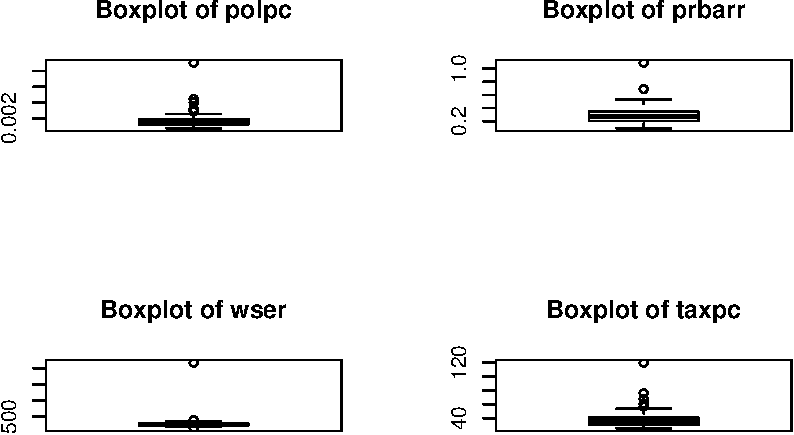
\includegraphics{Lab_3_files/figure-latex/unnamed-chunk-4-1.pdf}

\begin{Shaded}
\begin{Highlighting}[]
\KeywordTok{plot}\NormalTok{(crime_df}\OperatorTok{$}\NormalTok{west, crime_df}\OperatorTok{$}\NormalTok{pctmin80)}
\end{Highlighting}
\end{Shaded}

\includegraphics{Lab_3_files/figure-latex/unnamed-chunk-4-2.pdf}

\begin{Shaded}
\begin{Highlighting}[]
\KeywordTok{plot}\NormalTok{(crime_df}\OperatorTok{$}\NormalTok{wtrd, crime_df}\OperatorTok{$}\NormalTok{wfir)}
\end{Highlighting}
\end{Shaded}

\includegraphics{Lab_3_files/figure-latex/unnamed-chunk-4-3.pdf}

\begin{Shaded}
\begin{Highlighting}[]
\KeywordTok{plot}\NormalTok{(crime_df}\OperatorTok{$}\NormalTok{wtrd, crime_df}\OperatorTok{$}\NormalTok{wfed)}
\end{Highlighting}
\end{Shaded}

\includegraphics{Lab_3_files/figure-latex/unnamed-chunk-4-4.pdf}

\begin{Shaded}
\begin{Highlighting}[]
\KeywordTok{plot}\NormalTok{(crime_df}\OperatorTok{$}\NormalTok{wfed, crime_df}\OperatorTok{$}\NormalTok{wfir)}
\end{Highlighting}
\end{Shaded}

\includegraphics{Lab_3_files/figure-latex/unnamed-chunk-4-5.pdf}

\begin{Shaded}
\begin{Highlighting}[]
\KeywordTok{plot}\NormalTok{(crime_df}\OperatorTok{$}\NormalTok{wfed}\OperatorTok{+}\NormalTok{crime_df}\OperatorTok{$}\NormalTok{wtrd}\OperatorTok{+}\NormalTok{crime_df}\OperatorTok{$}\NormalTok{wfir, crime_df}\OperatorTok{$}\NormalTok{density)}
\end{Highlighting}
\end{Shaded}

\includegraphics{Lab_3_files/figure-latex/unnamed-chunk-4-6.pdf} \#\#\#
Standardize Independent Variables

In order to compare the impacts of the different independent variables,
the values of those variables needed to be standardized so that the
slope coefficients are similar in scale (e.g.~if the range of a variable
is between 0 and 1, then the coefficient may be larger than that of a
variable that ranges between 0-200). For the standardization, the
variables were all scaled to range between 0 and 1, based on the min and
max values.

\begin{Shaded}
\begin{Highlighting}[]
\CommentTok{# make a copy of crime_df for standardizing values}
\NormalTok{std_crime_df <-}\StringTok{ }\KeywordTok{cbind}\NormalTok{(crime_df)}

\CommentTok{# a function to standardize values (fraction of range)}
\NormalTok{standardize_values <-}\StringTok{ }\ControlFlowTok{function}\NormalTok{(x)\{(x}\OperatorTok{-}\KeywordTok{min}\NormalTok{(x))}\OperatorTok{/}\NormalTok{(}\KeywordTok{max}\NormalTok{(x)}\OperatorTok{-}\KeywordTok{min}\NormalTok{(x))\}}

\CommentTok{# for all columns other than county number, year, and crime rate, standardize between 0 and 1}
\ControlFlowTok{for}\NormalTok{ (col }\ControlFlowTok{in} \DecValTok{4}\OperatorTok{:}\KeywordTok{ncol}\NormalTok{(std_crime_df)) \{}
\NormalTok{  std_crime_df[,col] <-}\StringTok{ }\KeywordTok{standardize_values}\NormalTok{(std_crime_df[,col])}
\NormalTok{\}}

\KeywordTok{summary}\NormalTok{(std_crime_df)}
\end{Highlighting}
\end{Shaded}

\begin{verbatim}
##      county           year        crmrte             prbarr      
##  Min.   :  1.0   Min.   :87   Min.   :0.005533   Min.   :0.0000  
##  1st Qu.: 52.0   1st Qu.:87   1st Qu.:0.020927   1st Qu.:0.1131  
##  Median :105.0   Median :87   Median :0.029986   Median :0.1785  
##  Mean   :101.6   Mean   :87   Mean   :0.033400   Mean   :0.2025  
##  3rd Qu.:152.0   3rd Qu.:87   3rd Qu.:0.039642   3rd Qu.:0.2521  
##  Max.   :197.0   Max.   :87   Max.   :0.098966   Max.   :1.0000  
##     prbconv          prbpris           avgsen           polpc        
##  Min.   :0.0000   Min.   :0.0000   Min.   :0.0000   Min.   :0.00000  
##  1st Qu.:0.1350   1st Qu.:0.4773   1st Qu.:0.1279   1st Qu.:0.05837  
##  Median :0.1873   Median :0.6076   Median :0.2428   Median :0.08900  
##  Mean   :0.2352   Mean   :0.5795   Mean   :0.2785   Mean   :0.11510  
##  3rd Qu.:0.2535   3rd Qu.:0.6817   3rd Qu.:0.3943   3rd Qu.:0.13611  
##  Max.   :1.0000   Max.   :1.0000   Max.   :1.0000   Max.   :1.00000  
##     density            taxpc              west           central      
##  Min.   :0.00000   Min.   :0.00000   Min.   :0.0000   Min.   :0.0000  
##  1st Qu.:0.06201   1st Qu.:0.05283   1st Qu.:0.0000   1st Qu.:0.0000  
##  Median :0.10900   Median :0.09756   Median :0.0000   Median :0.0000  
##  Mean   :0.16186   Mean   :0.13142   Mean   :0.2527   Mean   :0.3736  
##  3rd Qu.:0.17765   3rd Qu.:0.16217   3rd Qu.:0.5000   3rd Qu.:1.0000  
##  Max.   :1.00000   Max.   :1.00000   Max.   :1.0000   Max.   :1.0000  
##      urban            pctmin80           wcon             wtuc       
##  Min.   :0.00000   Min.   :0.0000   Min.   :0.0000   Min.   :0.0000  
##  1st Qu.:0.00000   1st Qu.:0.1358   1st Qu.:0.2350   1st Qu.:0.4394  
##  Median :0.00000   Median :0.3652   Median :0.3611   Median :0.5143  
##  Mean   :0.08791   Mean   :0.3839   Mean   :0.3772   Mean   :0.5264  
##  3rd Qu.:0.00000   3rd Qu.:0.5845   3rd Qu.:0.4983   3rd Qu.:0.6011  
##  Max.   :1.00000   Max.   :1.0000   Max.   :1.0000   Max.   :1.0000  
##       wtrd             wfir             wser              wmfg       
##  Min.   :0.0000   Min.   :0.0000   Min.   :0.00000   Min.   :0.0000  
##  1st Qu.:0.1828   1st Qu.:0.3414   1st Qu.:0.04727   1st Qu.:0.2686  
##  Median :0.2435   Median :0.4324   Median :0.05880   Median :0.3326  
##  Mean   :0.2861   Mean   :0.4465   Mean   :0.06973   Mean   :0.3640  
##  3rd Qu.:0.3538   3rd Qu.:0.5152   3rd Qu.:0.07216   3rd Qu.:0.4131  
##  Max.   :1.0000   Max.   :1.0000   Max.   :1.00000   Max.   :1.0000  
##       wfed             wsta             wloc             mix        
##  Min.   :0.0000   Min.   :0.0000   Min.   :0.0000   Min.   :0.0000  
##  1st Qu.:0.2727   1st Qu.:0.2943   1st Qu.:0.3901   1st Qu.:0.1372  
##  Median :0.4552   Median :0.4118   Median :0.4625   Median :0.1846  
##  Mean   :0.4297   Mean   :0.4111   Mean   :0.4936   Mean   :0.2452  
##  3rd Qu.:0.5589   3rd Qu.:0.5150   3rd Qu.:0.6049   3rd Qu.:0.2966  
##  Max.   :1.0000   Max.   :1.0000   Max.   :1.0000   Max.   :1.0000  
##     pctymle       
##  Min.   :0.00000  
##  1st Qu.:0.06579  
##  Median :0.08338  
##  Mean   :0.11688  
##  3rd Qu.:0.11439  
##  Max.   :1.00000
\end{verbatim}

Now that we have standardized the units of all input variables, we can
compute model slope coefficients that will be in comparable units.

\subsubsection{Standardized Regression
Model}\label{standardized-regression-model}

A multi variable regression model was created using the data set that
has been standardized above.

Then the model was evaluated for potential high leverage/influence data
points as well as potential biases.

In review the following findings were noted: - row 84 and 25 have a high
Cook's distance and high standardized residuals, which means the data
point can be problematic for the regression model. - row 25 and 84 were
also noted earlier to be an extreme outier for the wser variable. Thus
based on this finding the point will be removed and the regression will
be redone. - Judging from the residuals vs.~fitted plot the model may
have some bias when the predicted value crmrte is between 0 to 0.04.
Particularly the model tend to underpredict lower crmrates, and
overpredict medium crmrte. - From the Normal Q-Q line, it looks like
that majority of predictions follow the line, indicating a normal and
independent distribution.

\begin{Shaded}
\begin{Highlighting}[]
\CommentTok{#TODO clean out the warning}
\NormalTok{std_model <-}\StringTok{ }\KeywordTok{lm}\NormalTok{(crmrte }\OperatorTok{~}\StringTok{ }\NormalTok{. }\OperatorTok{-}\StringTok{ }\NormalTok{county}\OperatorTok{-}\NormalTok{year}\OperatorTok{-}\NormalTok{crmrte}\OperatorTok{-}\NormalTok{urban}\OperatorTok{-}\NormalTok{west}\OperatorTok{-}\NormalTok{wtrd}\OperatorTok{-}\NormalTok{wfed}\OperatorTok{-}\NormalTok{wfir, }\DataTypeTok{data =}\NormalTok{  std_crime_df)}

\KeywordTok{plot}\NormalTok{(std_model)}
\end{Highlighting}
\end{Shaded}

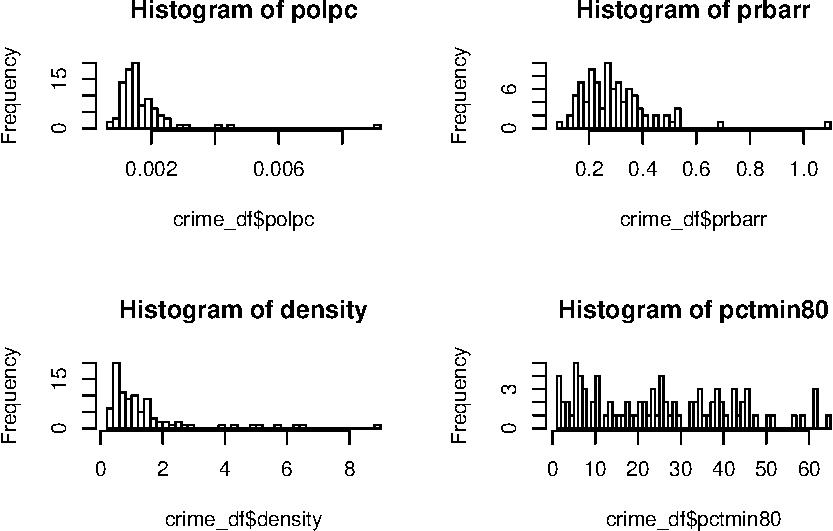
\includegraphics{Lab_3_files/figure-latex/unnamed-chunk-6-1.pdf}
\includegraphics{Lab_3_files/figure-latex/unnamed-chunk-6-2.pdf}
\includegraphics{Lab_3_files/figure-latex/unnamed-chunk-6-3.pdf}

\begin{verbatim}
## Warning in sqrt(crit * p * (1 - hh)/hh): NaNs produced

## Warning in sqrt(crit * p * (1 - hh)/hh): NaNs produced
\end{verbatim}

\includegraphics{Lab_3_files/figure-latex/unnamed-chunk-6-4.pdf}

\begin{Shaded}
\begin{Highlighting}[]
\CommentTok{#summary(std_model)$r.squared}
\end{Highlighting}
\end{Shaded}

\begin{Shaded}
\begin{Highlighting}[]
\NormalTok{std_crime_df2 <-}\StringTok{ }\NormalTok{std_crime_df[}\OperatorTok{-}\KeywordTok{c}\NormalTok{(}\DecValTok{84}\NormalTok{,}\DecValTok{25}\NormalTok{),]}

\NormalTok{std_model2 <-}\StringTok{ }\KeywordTok{lm}\NormalTok{(crmrte }\OperatorTok{~}\StringTok{ }\NormalTok{. }\OperatorTok{-}\StringTok{ }\NormalTok{county}\OperatorTok{-}\NormalTok{year}\OperatorTok{-}\NormalTok{crmrte}\OperatorTok{-}\NormalTok{urban}\OperatorTok{-}\NormalTok{west}\OperatorTok{-}\NormalTok{wtrd}\OperatorTok{-}\NormalTok{wfed}\OperatorTok{-}\NormalTok{wfir, }\DataTypeTok{data =}\NormalTok{  std_crime_df2)}

\KeywordTok{plot}\NormalTok{(std_model2)}
\end{Highlighting}
\end{Shaded}

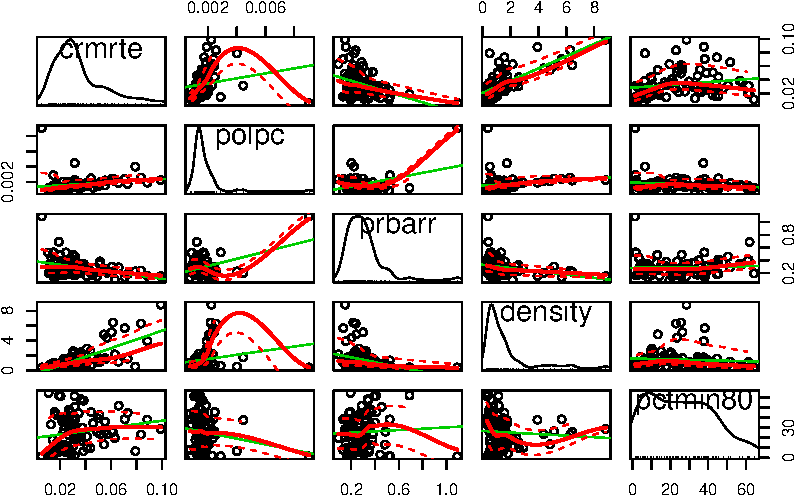
\includegraphics{Lab_3_files/figure-latex/unnamed-chunk-7-1.pdf}
\includegraphics{Lab_3_files/figure-latex/unnamed-chunk-7-2.pdf}
\includegraphics{Lab_3_files/figure-latex/unnamed-chunk-7-3.pdf}
\includegraphics{Lab_3_files/figure-latex/unnamed-chunk-7-4.pdf}

In order to find which variables are most impactful to crmrte, the
marginal R-squared against the standardized coefficients were reviewed.
Based on the plots, the following variables were found to have the
highest marginal R-squared and absolute slope coefficient: -prbarr
-prbconv -polpc -density -pctmin80

\begin{Shaded}
\begin{Highlighting}[]
\NormalTok{coeff_df =}\StringTok{ }\KeywordTok{data.frame}\NormalTok{(}\KeywordTok{summary}\NormalTok{(std_model)}\OperatorTok{$}\NormalTok{coefficients)}
\CommentTok{#summary(std_model)$r.squared}

\CommentTok{#base R-Squared}
\NormalTok{base_model <-}\StringTok{ }\KeywordTok{lm}\NormalTok{(crmrte}\OperatorTok{~}\NormalTok{.}\OperatorTok{-}\NormalTok{county}\OperatorTok{-}\NormalTok{year}\OperatorTok{-}\NormalTok{crmrte, }\DataTypeTok{data=}\NormalTok{std_crime_df)}
\NormalTok{base_r2 <-}\StringTok{ }\KeywordTok{summary}\NormalTok{(base_model)}\OperatorTok{$}\NormalTok{r.squared}

\CommentTok{#create list of variables for the for-loop}
\NormalTok{var_names <-}\StringTok{ }\KeywordTok{colnames}\NormalTok{(std_crime_df)}
\NormalTok{remove <-}\StringTok{ }\KeywordTok{c}\NormalTok{(}\StringTok{'county'}\NormalTok{,}
            \StringTok{'year'}\NormalTok{,}
            \StringTok{'crmrte'}\NormalTok{,}
            \StringTok{'urban'}\NormalTok{,}
            \StringTok{'west'}\NormalTok{,}
            \StringTok{'wtrd'}\NormalTok{,}
            \StringTok{'wfed'}\NormalTok{,}
            \StringTok{'wfir'}\NormalTok{)}
\NormalTok{var_names <-}\StringTok{ }\NormalTok{var_names[}\OperatorTok{!}\StringTok{ }\NormalTok{var_names }\OperatorTok\StringTok{ }\NormalTok{remove]}

\CommentTok{#initiate an empty vector to store the marginal R-Squared}
\NormalTok{var_r2_delta =}\StringTok{ }\KeywordTok{c}\NormalTok{()}

\CommentTok{#loop through the variable names and store the marginal R-Squared}
\ControlFlowTok{for}\NormalTok{ (i }\ControlFlowTok{in}\NormalTok{ var_names) \{}
\NormalTok{    fmla <-}\StringTok{ }\KeywordTok{as.formula}\NormalTok{(}\KeywordTok{paste}\NormalTok{(}\StringTok{"crmrte ~ - crmrte +"}\NormalTok{, }\KeywordTok{paste}\NormalTok{(var_names[}\OperatorTok{!}\StringTok{ }\NormalTok{var_names }\OperatorTok\StringTok{ }\NormalTok{i], }\DataTypeTok{collapse=} \StringTok{"+"}\NormalTok{)))}
\NormalTok{    delta_model <-}\StringTok{ }\KeywordTok{lm}\NormalTok{(fmla, }\DataTypeTok{data=}\NormalTok{crime_df)}
\NormalTok{    r2_delta <-}\StringTok{ }\NormalTok{base_r2}\OperatorTok{-}\KeywordTok{summary}\NormalTok{(delta_model)}\OperatorTok{$}\NormalTok{r.squared}
\NormalTok{    var_r2_delta <-}\StringTok{ }\KeywordTok{c}\NormalTok{(var_r2_delta, r2_delta)}
\NormalTok{\}}

\CommentTok{#put the variable and marginal R-squared in a dataframe}
\NormalTok{mar_r2_df <-}\StringTok{ }\KeywordTok{data.frame}\NormalTok{(}\DataTypeTok{v1=}\NormalTok{var_names, }\DataTypeTok{v2=}\NormalTok{var_r2_delta)}
\KeywordTok{colnames}\NormalTok{(mar_r2_df) <-}\StringTok{ }\KeywordTok{c}\NormalTok{(}\StringTok{'variable'}\NormalTok{, }\StringTok{'marginalr2'}\NormalTok{)}

\CommentTok{#sort dataframe by marginal R-squared in a descending order}
\CommentTok{#mar_r2_df <- mar_r2_df[rev(order(mar_r2_df$marginalr2)),]}

\KeywordTok{plot}\NormalTok{(}\KeywordTok{abs}\NormalTok{(coeff_df[}\OperatorTok{-}\KeywordTok{c}\NormalTok{(}\DecValTok{1}\NormalTok{),]}\OperatorTok{$}\NormalTok{Estimate),mar_r2_df}\OperatorTok{$}\NormalTok{marginalr2)}
\end{Highlighting}
\end{Shaded}

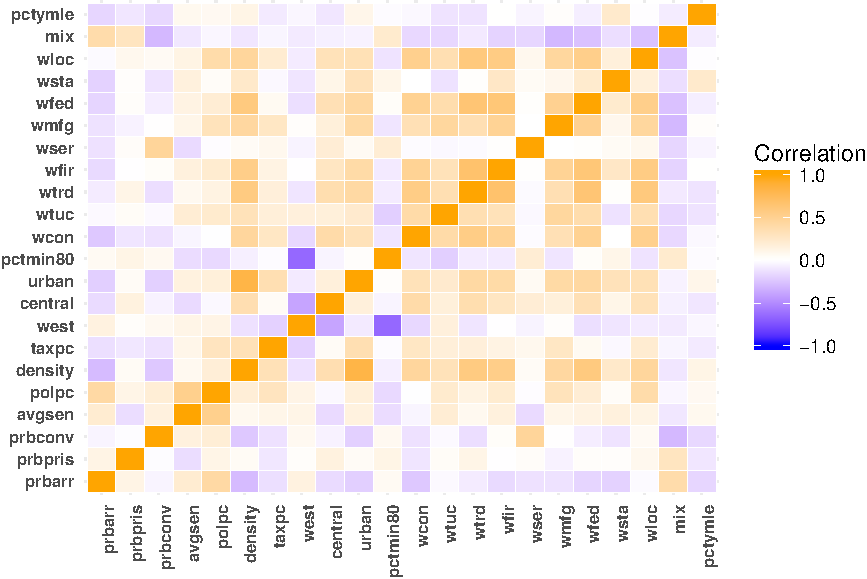
\includegraphics{Lab_3_files/figure-latex/unnamed-chunk-8-1.pdf}

\begin{Shaded}
\begin{Highlighting}[]
\KeywordTok{subset}\NormalTok{(mar_r2_df, marginalr2 }\OperatorTok{>}\StringTok{ }\NormalTok{.}\DecValTok{04}\NormalTok{)}
\end{Highlighting}
\end{Shaded}

\begin{verbatim}
##   variable marginalr2
## 1   prbarr 0.07445392
## 2  prbconv 0.07695649
## 5    polpc 0.05856302
## 6  density 0.10492397
## 9 pctmin80 0.11132549
\end{verbatim}

\subsubsection{Non-Standardized
Regressions}\label{non-standardized-regressions}

The following is the model that contains almost all available variables
as explanatory variables with the exception of variables we excluded due
to potential multi-collinearity.

\begin{Shaded}
\begin{Highlighting}[]
\NormalTok{crime_df2 <-}\StringTok{ }\NormalTok{crime_df[}\OperatorTok{-}\KeywordTok{c}\NormalTok{(}\DecValTok{84}\NormalTok{,}\DecValTok{25}\NormalTok{),]}

\NormalTok{model1 <-}\StringTok{ }\KeywordTok{lm}\NormalTok{(crmrte }\OperatorTok{~}\StringTok{ }\NormalTok{. }\OperatorTok{-}\StringTok{ }\NormalTok{county}\OperatorTok{-}\NormalTok{year}\OperatorTok{-}\NormalTok{crmrte}\OperatorTok{-}\NormalTok{urban}\OperatorTok{-}\NormalTok{west}\OperatorTok{-}\NormalTok{wtrd}\OperatorTok{-}\NormalTok{wfed}\OperatorTok{-}\NormalTok{wfir, }\DataTypeTok{data =}\NormalTok{ crime_df2)}

\KeywordTok{summary}\NormalTok{(model1)}\OperatorTok{$}\NormalTok{r.squared}
\end{Highlighting}
\end{Shaded}

\begin{verbatim}
## [1] 0.8688977
\end{verbatim}

\begin{Shaded}
\begin{Highlighting}[]
\KeywordTok{summary}\NormalTok{(model1)}\OperatorTok{$}\NormalTok{coefficients}
\end{Highlighting}
\end{Shaded}

\begin{verbatim}
##                  Estimate   Std. Error    t value     Pr(>|t|)
## (Intercept)  3.097640e-02 1.561081e-02  1.9842914 5.108937e-02
## prbarr      -5.078247e-02 8.704418e-03 -5.8341022 1.478721e-07
## prbconv     -1.962352e-02 3.293124e-03 -5.9589361 8.903946e-08
## prbpris      4.754774e-03 1.048442e-02  0.4535087 6.515656e-01
## avgsen      -3.961756e-04 3.497705e-04 -1.1326727 2.611624e-01
## polpc        6.460940e+00 1.346144e+00  4.7995886 8.534766e-06
## density      6.845704e-03 7.973078e-04  8.5860246 1.369694e-12
## taxpc       -7.103721e-05 1.021711e-04 -0.6952767 4.891513e-01
## central     -3.517708e-03 1.926533e-03 -1.8259265 7.206619e-02
## pctmin80     3.898315e-04 5.176540e-05  7.5307361 1.236934e-10
## wcon         4.081808e-05 2.373695e-05  1.7196007 8.986184e-02
## wtuc         4.373842e-06 1.324754e-05  0.3301626 7.422493e-01
## wser        -6.293562e-05 2.794740e-05 -2.2519307 2.742112e-02
## wmfg         4.568252e-06 1.208881e-05  0.3778909 7.066390e-01
## wsta        -4.273992e-05 2.105298e-05 -2.0301130 4.609284e-02
## wloc         4.531803e-05 4.143979e-05  1.0935875 2.778324e-01
## mix         -2.294321e-02 1.269191e-02 -1.8077035 7.488831e-02
## pctymle      9.580106e-02 3.779334e-02  2.5348663 1.345432e-02
\end{verbatim}

The following is the model that contains a transformed explanatory
variable.

\begin{Shaded}
\begin{Highlighting}[]
\NormalTok{model_transform <-}\StringTok{ }\KeywordTok{lm}\NormalTok{(crmrte }\OperatorTok{~}\StringTok{ }\NormalTok{prbarr }\OperatorTok{+}\StringTok{ }\KeywordTok{log}\NormalTok{(prbconv) }\OperatorTok{+}\StringTok{ }\NormalTok{density, }\DataTypeTok{data =}\NormalTok{ crime_df2)}

\KeywordTok{summary}\NormalTok{(model_transform)}\OperatorTok{$}\NormalTok{r.squared}
\end{Highlighting}
\end{Shaded}

\begin{verbatim}
## [1] 0.6570935
\end{verbatim}

\begin{Shaded}
\begin{Highlighting}[]
\KeywordTok{summary}\NormalTok{(model_transform)}\OperatorTok{$}\NormalTok{coefficients}
\end{Highlighting}
\end{Shaded}

\begin{verbatim}
##                  Estimate   Std. Error   t value     Pr(>|t|)
## (Intercept)   0.025420503 0.0035106022  7.241066 1.857260e-10
## prbarr       -0.028710438 0.0089889944 -3.193954 1.969045e-03
## log(prbconv) -0.006276946 0.0022761837 -2.757662 7.125235e-03
## density       0.007903815 0.0008331222  9.486981 5.580124e-15
\end{verbatim}

The following is the model that contains only variables that were
identified to be most relevant to crmrte based on their marginal
R-squared and standardized slope coefficient values.

\begin{Shaded}
\begin{Highlighting}[]
\NormalTok{model_key <-}\StringTok{ }\KeywordTok{lm}\NormalTok{(crmrte }\OperatorTok{~}\StringTok{ }\NormalTok{prbarr }\OperatorTok{+}\StringTok{ }\NormalTok{prbconv }\OperatorTok{+}\StringTok{ }\NormalTok{polpc }\OperatorTok{+}\StringTok{ }\NormalTok{density }\OperatorTok{+}\StringTok{ }\NormalTok{pctmin80, }\DataTypeTok{data =}\NormalTok{ crime_df2)}

\KeywordTok{summary}\NormalTok{(model_key)}\OperatorTok{$}\NormalTok{r.squared}
\end{Highlighting}
\end{Shaded}

\begin{verbatim}
## [1] 0.8204393
\end{verbatim}

\begin{Shaded}
\begin{Highlighting}[]
\KeywordTok{summary}\NormalTok{(model_key)}\OperatorTok{$}\NormalTok{coefficients}
\end{Highlighting}
\end{Shaded}

\begin{verbatim}
##                  Estimate   Std. Error   t value     Pr(>|t|)
## (Intercept)  0.0300488820 3.494735e-03  8.598328 4.156915e-13
## prbarr      -0.0555832603 8.317408e-03 -6.682763 2.515871e-09
## prbconv     -0.0179293179 3.139371e-03 -5.711118 1.698543e-07
## polpc        6.1601721055 1.204450e+00  5.114512 1.989594e-06
## density      0.0063705861 6.966292e-04  9.144873 3.349488e-14
## pctmin80     0.0003808799 5.212093e-05  7.307620 1.527153e-10
\end{verbatim}

\subsubsection{Recommendation}\label{recommendation}

For interpretability purposes, the model was re-done using
non-standardized variables: -prbarr -prbconv -polpc -density -pctmin80

Recommendation for political campaign: - police per capita has a
positive slope coefficient with crmrte, and this may be due to more
police are present in areas with high crmrte. This suggests that purely
hiring more police officers may not be an impactful solution. - However
probability of arrest and conviction both have a negative slope
coefficients. The model suggests that perhaps a zero tolerance policy
towards crime is needed to increase arrests and convictions and thus
deter crimes from happening. - In terms areas with large minority
population and high density, since these variable cannot be changed that
much, perhaps a community outreach (e.g.~job training program,
afterschool programs, tutor/mentor program) to educate areas with a lot
of minority can be done, so that crimes can be reduced in those areas.

\subsubsection{Omitted Variables}\label{omitted-variables}

Potential Omitted Variable \#1: poverty\_rate
\[ crmrte = \beta_0 + \beta_1*density + \beta_2*poverty\_rate + u\]
\[ poverty\_rate = \alpha_0 + \alpha_1*density +u \]

\begin{itemize}
\tightlist
\item
  One thing that was noticeable in the data is that crmrate was higher
  in dense areas and large minority population, however this may be due
  to an omitted variable that is not available in the data set.
\item
  For example: in dense areas the cost of living may be much higher,
  which can explain why higher wages are correlated with dense areas,
  but because of the higher cost of living. Because of this, there may
  be a lot more people living under the poverty line, which would
  encourage them to commit crimes and hence why dense areas have higher
  crmrte.
\item
  so the density slope coefficient in this instance is probably higher
  than it should be \(\beta_2\) and \(\alpha_1\) would be positive.
\end{itemize}

Potential Omitted Variable \#2: discrimination
\[ crmrte = \beta_0 + \beta_1*pctmin80 + \beta_2*discrimination \]
\[ discrimination = \alpha_0 + \alpha_1*pctmin80 \] - Similarly
minorities may be arrested for crimes more often than necessary due to
discrimination. - in this scenario \(\beta_2\) and \(alpha_1\) would be
a positive value.

Potential Omitted Variable \#3: raised\_in\_oneparent\_hh
\[ crmrte = \beta_0 + \beta_1*pctmin80 + \beta_2*raised\_in\_2parents\_hh \]
\[ raised\_in\_2parents\_hh = \alpha_0 + \alpha_1*pctmin80 \] - In this
scenario, minorities may be more likely to be raised in a single parent
house hold. Thus making them more likely to commit crimes. - \(\beta_2\)
would be positive and \(\alpha_1\) would be negative.


\end{document}
